% =========================================================================
\section{Introdução e modelagem}
% =========================================================================

Este trabalho compara três abordagens para o sequenciamento da manutenção
preventiva de $n$ ativos por uma única equipe: \textit{greedy descent} com
\textit{random restart} (GD), \textit{simulated annealing} (SA) e um
\textit{genetic algorithm} (GA)~\cite{poole2023,russell2016,eiben2003}. Uma solução é uma permutação
$\pi=(\pi_1,\dots,\pi_n)$ (a ordem de visita), e o custo a minimizar é o atraso
ponderado total
\begin{equation}
h(\pi)=\sum_{j=1}^{n} w_j\max(0,\,C_j-d_j),\qquad
C_{\pi_k}=C_{\pi_{k-1}}+t_{\pi_{k-1}\pi_k}+p_{\pi_k},
\end{equation}
com deslocamentos $t_{ij}$ iguais à distância euclidiana arredondada para o
inteiro mais próximo. As três instâncias têm $n=12$, $50$ e $150$ ativos.

\textbf{Arquitetura.} O código separa algoritmo e problema
(\texttt{src/base.py}). Os algoritmos só chamam \texttt{solucao\_aleatoria},
\texttt{h}, \texttt{sucessores}, \texttt{sucessor\_aleatorio},
\texttt{aplicar}, \texttt{cruzamento}, \texttt{mutacao} e
\texttt{distancia}. Toda avaliação de $h$ passa por um único método
(\texttt{\_contar}), que incrementa o contador, lança uma exceção quando o
orçamento $B$ é atingido (a execução para \emph{exatamente} em $B$) e registra a
curva de convergência. Os três algoritmos não contêm nenhuma referência a
ativos, prazos ou tempos.

\textbf{T1: validação de $h$.} A saída do programa
(\texttt{python3 src/experimentos.py t1}) reproduz os valores de verificação:
\begin{verbatim}
pequena: h(identidade) = 4366
pequena: guloso (menor acréscimo de atraso) = 3168
pequena: ótimo exato (PD com fronteira de Pareto) = 1875,
         pi* = (5, 4, 1, 6, 7, 2, 8, 12, 3, 10, 9, 11)
\end{verbatim}
O exemplo da Figura~1 do enunciado ($h=39$ e $h^\star=22$) também é verificado
em teste automático (\texttt{tests/test\_manutencao.py}). Dois detalhes
merecem registro:
\begin{itemize}
    \item o guloso só reproduz 3168 quando os empates em ``menor acréscimo de
    atraso'' (frequentes no início, quando o acréscimo é zero) são desfeitos
    pelo ativo \emph{mais próximo}; desempatando pelo menor índice, ele dá 6935;
    \item o ótimo 1875 foi confirmado de forma independente por programação
    dinâmica sobre (conjunto visitado, último ativo), mantendo a fronteira de
    Pareto de (tempo, custo). Essa busca exata mostrou que o ótimo global é
    único.
\end{itemize}

% =========================================================================
\section{Vizinhanças e avaliação incremental (T2)}
% =========================================================================

Os três operadores (\textit{swap}, \textit{insertion} e \textit{2-opt})
induzem vizinhanças de tamanho $n(n-1)/2$, $(n-1)^2$ e $n(n-1)/2$,
respectivamente. Na \textit{insertion}, mover o ativo da posição $i$ para
$i+1$ produz a mesma sequência que mover o de $i+1$ para $i$; descontadas essas
$n-1$ duplicatas, sobram $(n-1)^2$ vizinhos distintos, o que foi conferido em
teste. Para $n=150$ isso dá \num{11175}, \num{22201} e \num{11175} sucessores.

\textbf{Avaliação incremental.} Um movimento que altera apenas as posições
$a..b$ mantém o prefixo $\pi_1..\pi_{a-1}$, cujo custo e tempo de conclusão
são lidos do cronograma já calculado para $\pi$. Recalcula-se só o trecho
$a..b$. Da posição $b+1$ em diante os ativos são os mesmos, e todos sofrem o
mesmo deslocamento de tempo $\delta$. Assim, o custo do sufixo é
$\sum_{k>b} w_k\max(0,\delta-f_k)$, com folgas $f_k=d_k-C_k$ pré-calculadas; se
$\delta=0$, o sufixo custa o mesmo que antes. Como $h$ é não decrescente ao
longo do prefixo, a soma é interrompida quando ultrapassa um limite (o $h$ da
solução corrente). Um valor interrompido só é usado para rejeitar o
movimento, nunca é reportado.

Um teste automático compara a avaliação incremental com a completa em
\num{5400} movimentos das três vizinhanças, nas três instâncias, com e sem
limite. Dentro de uma descida \textit{first improvement}, a avaliação
incremental reduziu o tempo por sucessor de \SI{12}{\micro\second} para
\SI{8}{\micro\second} em $n=150$ (ganho de cerca de $1{,}5\times$). Em $n=12$
não houve ganho: o custo fixo do Python domina e o sufixo é curto demais para
compensar (\autoref{table:t2}). A contagem de avaliações não muda, e
verificamos que a trajetória da busca é idêntica nos dois modos.

\begin{table}[H]
    \centering
    \caption{T2: GD com \textit{random restart} em cada vizinhança (10
    execuções, mesmo orçamento da Seção~3). A coluna $p$ é o teste de
    Mann--Whitney contra a melhor vizinhança na variante \textit{first}. As
    colunas de tempo medem o custo por sucessor dentro de uma descida
    \textit{first improvement}.}
    \label{table:t2}
    \begin{adjustbox}{max width=\linewidth}
    \begin{tabular}{llrrrrrr}
\toprule
 & & \multicolumn{3}{c}{mediana do melhor $h$ (10 exec.)} & \multicolumn{3}{c}{$\mu$s por sucessor} \\
\cmidrule(lr){3-5}\cmidrule(lr){6-8}
Instância & Vizinhança & Best & First & $p$ (First) & completa & incremental & ganho \\
\midrule
Pequena ($n=12$) & Swap & 1\,875 & \textbf{1\,875} & -- & 1,7 & 1,6 & 1,02$\times$ \\
 & Insertion & 1\,875 & 1\,875 & 1,000 & 1,6 & 1,5 & 1,06$\times$ \\
 & 2-opt & 1\,875 & 1\,875 & 1,000 & 1,7 & 1,6 & 1,03$\times$ \\
\midrule
Intermediária ($n=50$) & Swap & 30\,896 & 25\,690 & 0,0002 & 4,6 & 3,0 & 1,51$\times$ \\
 & Insertion & 20\,326 & \textbf{17\,408} & -- & 4,4 & 3,1 & 1,40$\times$ \\
 & 2-opt & 20\,514 & 18\,502 & 0,121 & 4,4 & 3,0 & 1,45$\times$ \\
\midrule
Grande ($n=150$) & Swap & 468\,855 & 150\,198 & 0,0002 & 12,7 & 8,3 & 1,54$\times$ \\
 & Insertion & 821\,542 & \textbf{81\,175} & -- & 11,9 & 8,1 & 1,48$\times$ \\
 & 2-opt & 473\,487 & 95\,346 & 0,0003 & 11,9 & 7,6 & 1,56$\times$ \\
\bottomrule
\end{tabular}

    \end{adjustbox}
\end{table}

Na instância pequena as três vizinhanças empatam (todas chegam a 1875). Nas
maiores, a \textbf{\textit{insertion}} produz os melhores ótimos locais com
\textit{first improvement}:
\begin{itemize}
    \item $n=50$: mediana \num{17408}, contra \num{18502} do \textit{2-opt} e
    \num{25690} do \textit{swap};
    \item $n=150$: mediana \num{81175}, contra \num{95346} e \num{150198}, com
    $p<0{,}001$ nas duas comparações.
\end{itemize}

A explicação está na estrutura do problema. O custo depende de \emph{quando}
cada ativo é atendido, e a \textit{insertion} adianta ou atrasa um único ativo
deslocando os demais de apenas uma posição. O \textit{swap} troca dois ativos
de lugar e altera ao mesmo tempo dois deslocamentos de cada lado. O
\textit{2-opt} inverte um trecho inteiro, o que destrói a ordem por prazo que
as boas soluções têm.

Por sucessor, as três vizinhanças custam praticamente o mesmo
(\SIrange{7,6}{8,3}{\micro\second} em $n=150$). Por \emph{varredura completa},
porém, a \textit{insertion} custa o dobro, e isso a torna a pior opção para
\textit{best improvement} em $n=150$: a mediana chega a \num{821542}, porque
cada passo consome \num{22201} avaliações. \textbf{Adotamos a
\textit{insertion} nos demais experimentos.}

% =========================================================================
\section{Algoritmos e parâmetros}
% =========================================================================

\textbf{(A) GD com \textit{random restart}.} Implementamos as três variantes:
\begin{itemize}
    \item \textit{best improvement}: varre toda a vizinhança e move para o
    melhor sucessor;
    \item \textit{first improvement}: varre a vizinhança em ordem aleatória e
    aceita o primeiro sucessor que melhora;
    \item \textit{sucessor aleatório}: sorteia um sucessor e o aceita se
    melhorar. Como essa variante não consegue provar que está num ótimo local,
    declara-se ótimo local após $|N(\pi)|$ sorteios seguidos sem melhora.
\end{itemize}
Ao atingir o ótimo local, recomeça-se de uma permutação aleatória.

\textbf{(B) SA.} Aceita $\pi'$ se $h(\pi')\le h(\pi)$; caso contrário, aceita
com probabilidade $e^{-\Delta/T}$~\cite{poole2023}. O resfriamento é geométrico, com
$T\leftarrow\alpha T$ a cada avaliação, e os três parâmetros são definidos
assim:
\begin{itemize}
    \item \textbf{$T_0$} é calibrado \emph{na própria instância}: sorteiam-se
    200 sucessores da solução inicial (essas avaliações contam no orçamento) e
    escolhe-se $T_0$ tal que a piora média $\bar\Delta^+$ seja aceita com
    probabilidade $\chi_0$, isto é, $T_0=-\bar\Delta^+/\ln\chi_0$. Isso resolve
    o problema de escala apontado no enunciado: o $T_0$ mediano foi 941 na
    pequena, \num{14822} na intermediária e \num{5852} na grande;
    \item \textbf{$T_f$} é absoluto. Como $h$ é inteiro, a menor piora possível
    é 1, e com $T_f\le1$ uma piora de 5 é aceita com probabilidade menor que
    $0{,}7\%$, ou seja, o final é praticamente \textit{greedy descent};
    \item \textbf{$\alpha=(T_f/T_0)^{1/B'}$}, em que $B'$ é o orçamento
    restante, de modo que o resfriamento termine exatamente no fim do
    orçamento.
\end{itemize}
$\chi_0\in\{0{,}2;0{,}5;0{,}8\}$ e $T_f\in\{0{,}2;1;5\}$ foram escolhidos numa
calibração com 5 execuções por par e sementes distintas das do experimento
principal (Anexo~\ref{anexo:calib}). Resultado: $\chi_0=0{,}8$ e $T_f=1$ na
intermediária, $\chi_0=0{,}2$ e $T_f=0{,}2$ na grande, e $\chi_0=0{,}5$ e $T_f=1$
na pequena, onde todas as configurações empatam.

\textbf{(C) GA.} O algoritmo é geracional, com elitismo de 2 indivíduos,
$N=50$, $P_c=0{,}9$ e $P_m=0{,}5$, e a população inicial é aleatória. Os
operadores são:
\begin{itemize}
    \item \textbf{seleção:} torneio de tamanho 3. Como o torneio só compara
    indivíduos, basta declarar vencedor o de \emph{menor} $h$; não é preciso
    converter custo em aptidão, ao contrário da roleta, que exigiria algo como
    $f=1/(1+h)$ ou $f=h_{\max}-h$;
    \item \textbf{cruzamento:} \textit{Order Crossover} (OX)~\cite{eiben2003,gaspar2013}, detalhado abaixo;
    \item \textbf{mutação:} por \textit{insertion}, que na calibração
    (Anexo~\ref{anexo:calib}) foi muito superior à \textit{swap mutation} em
    todas as instâncias. Por exemplo, a mediana em $n=50$ foi \num{17704}
    contra \num{26022}.
\end{itemize}
Um filho que não sofreu cruzamento nem mutação herda o $h$ do pai sem gastar
avaliação.

\textit{Exemplo do OX (cortes nas posições 4 e 7):} pais
$p_1=(1\,2\,3\,\mathbf{4\,5\,6\,7}\,8\,9)$ e
$p_2=(9\,3\,7\,8\,2\,6\,5\,1\,4)$.
\begin{enumerate}
    \item O filho copia o trecho de $p_1$ nas mesmas posições:
    $(\_\,\_\,\_\,4\,5\,6\,7\,\_\,\_)$.
    \item Lê-se $p_2$ a partir da posição seguinte ao 2.º corte, circularmente:
    $1\,4\,9\,3\,7\,8\,2\,6\,5$.
    \item Removem-se os genes já presentes (4, 5, 6 e 7), o que deixa
    $1\,9\,3\,8\,2$.
    \item Esses genes preenchem as posições livres a partir da 8, também
    circularmente: posição 8 $\leftarrow1$, 9 $\leftarrow9$, 1 $\leftarrow3$,
    2 $\leftarrow8$, 3 $\leftarrow2$.
\end{enumerate}
O filho é $(3\,8\,2\,4\,5\,6\,7\,1\,9)$, uma permutação válida que preserva o
bloco de $p_1$ e a \emph{ordem relativa} de $p_2$. Esse exemplo é um teste
automático do código.

% =========================================================================
\section{Resultados (T3)}
% =========================================================================

Seguimos o protocolo da Seção~3: orçamento de \num{50000}, \num{150000} e
\num{300000} avaliações, com 30, 30 e 10 execuções independentes por
combinação. Cada execução tem semente própria, e as mesmas sementes são usadas
por todos os algoritmos. Reportamos as três variantes do GD; nas figuras,
``GD'' se refere ao \textit{first improvement}, que é a melhor variante.

\begin{table}[H]
    \centering
    \caption{Melhor $h$ por combinação. ``Gap'' é $(h-h^\star)/h^\star$ com
    $h^\star=1875$. ``Passos'' são os movimentos de melhoria aceitos (mediana).
    Tempo médio de parede por execução; os 8 processos rodaram em paralelo.}
    \label{table:principal}
    \begin{adjustbox}{max width=\linewidth}
    \begin{tabular}{llrrrrrr}
\toprule
Instância & Algoritmo & média $\pm$ desvio & mínimo & mediana & gap médio & tempo (s) & passos \\
\midrule
Pequena ($n=12$) & GD best & 1\,875 $\pm$ 0 & 1\,875 & 1\,875 & 0,0\% & 0,1 & 363 \\
 & GD first & 1\,875 $\pm$ 0 & 1\,875 & 1\,875 & 0,0\% & 0,1 & 2\,396 \\
 & GD aleatório & 1\,875 $\pm$ 0 & 1\,875 & 1\,875 & 0,0\% & 0,1 & 2\,519 \\
 & SA & 1\,875 $\pm$ 0 & 1\,875 & 1\,875 & 0,0\% & 0,2 & -- \\
 & GA & 2\,002 $\pm$ 154 & 1\,875 & 1\,937 & 6,8\% & 1,0 & -- \\
\midrule
Intermediária ($n=50$) & GD best & 21\,111 $\pm$ 2\,262 & 17\,451 & 20\,690 & -- & 0,7 & 61 \\
 & GD first & 17\,102 $\pm$ 584 & 16\,234 & 16\,920 & -- & 0,7 & 1\,687 \\
 & GD aleatório & 17\,392 $\pm$ 757 & 16\,242 & 17\,466 & -- & 0,8 & 1\,775 \\
 & SA & 16\,831 $\pm$ 507 & 16\,235 & 16\,681 & -- & 1,2 & -- \\
 & GA & 19\,548 $\pm$ 1\,967 & 16\,498 & 19\,636 & -- & 5,6 & -- \\
\midrule
Grande ($n=150$) & GD best & 817\,733 $\pm$ 24\,398 & 788\,457 & 809\,608 & -- & 3,4 & 13 \\
 & GD first & 82\,448 $\pm$ 7\,270 & 73\,413 & 82\,655 & -- & 3,2 & 1\,226 \\
 & GD aleatório & 81\,547 $\pm$ 6\,230 & 71\,109 & 82\,441 & -- & 3,5 & 1\,272 \\
 & SA & 71\,812 $\pm$ 5\,847 & 64\,519 & 71\,064 & -- & 4,3 & -- \\
 & GA & 89\,739 $\pm$ 8\,316 & 76\,266 & 91\,501 & -- & 22,4 & -- \\
\bottomrule
\end{tabular}

    \end{adjustbox}
\end{table}

\begin{figure}[H]
    \centering
    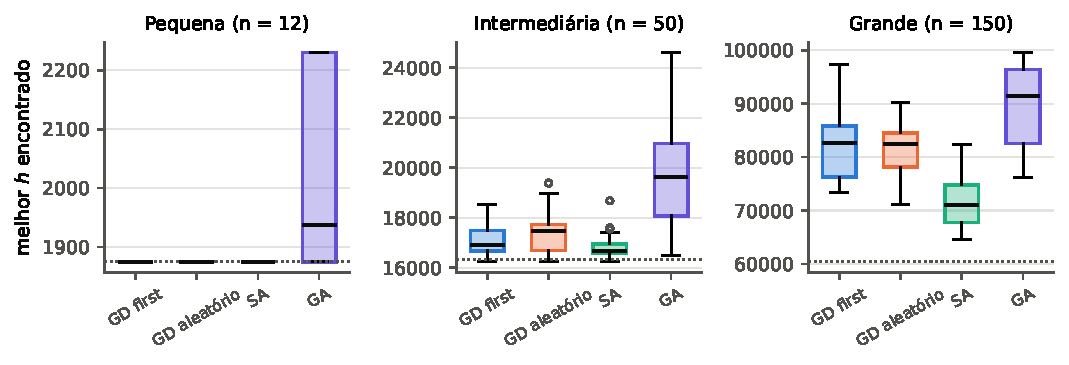
\includegraphics[width=\linewidth]{figures/tp2/boxplots.pdf}
    \caption{Distribuição do melhor $h$ por algoritmo. A linha pontilhada é o
    valor de referência (ótimo em $n=12$; melhor conhecido nas demais). O GD
    \textit{best} fica fora da escala em $n=150$ (\num{817733} em média).}
    \label{fig:box}
\end{figure}

\begin{table}[H]
    \centering
    \caption{Testes de Mann--Whitney bilaterais sobre o melhor $h$. Entre
    parênteses, o sinal da comparação entre as medianas (primeiro algoritmo
    versus segundo). ``Idênticos'' indica que todas as execuções deram 1875.}
    \label{table:testes}
    \begin{adjustbox}{max width=\linewidth}
    \begin{tabular}{lrrr}
\toprule
Comparação & Pequena ($n=12$) & Intermediária ($n=50$) & Grande ($n=150$) \\
\midrule
SA vs GD first & idênticos & 0,048 (<) & 0,0028 (<) \\
SA vs GD aleatório & idênticos & 0,0018 (<) & 0,0058 (<) \\
GD first vs GD aleatório & idênticos & 0,160 (<) & 0,910 (>) \\
GD first vs GD best & idênticos & $<10^{-4}$ (<) & 0,0002 (<) \\
SA vs GA & $<10^{-4}$ (<) & $<10^{-4}$ (<) & 0,0006 (<) \\
GD first vs GA & $<10^{-4}$ (<) & $<10^{-4}$ (<) & 0,054 (<) \\
\bottomrule
\end{tabular}

    \end{adjustbox}
\end{table}

\begin{figure}[H]
    \centering
    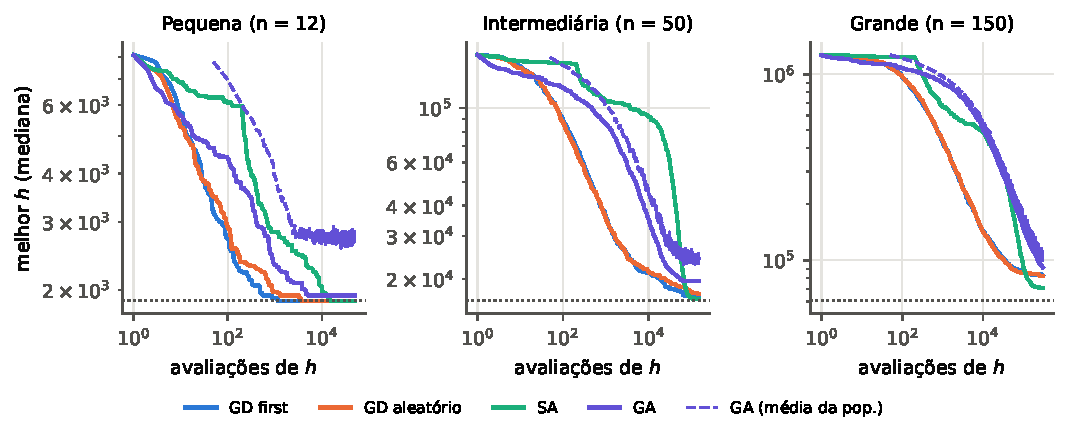
\includegraphics[width=\linewidth]{figures/tp2/convergencia.pdf}
    \caption{Curvas de convergência: mediana, entre execuções, do melhor $h$
    em função das avaliações (eixos logarítmicos). A curva tracejada é a
    mediana da \emph{média da população} do GA.}
    \label{fig:conv}
\end{figure}

\textbf{Tempo $\times$ avaliações.} Com o mesmo orçamento de avaliações, o GA
gasta 22\,s por execução em $n=150$, contra 3--4\,s da busca local e do SA
(\autoref{table:principal}). São cerca de \SI{75}{\micro\second} por
avaliação no GA contra \SI{11}{\micro\second} no GD. A diferença tem três
causas:
\begin{itemize}
    \item cada filho do GA exige uma avaliação \emph{completa} $O(n)$, sem a
    incremental;
    \item o cruzamento OX também custa $O(n)$;
    \item a diversidade da população é medida a cada geração.
\end{itemize}
Contar avaliações iguala o acesso à função objetivo, mas não iguala o custo
computacional. Se o critério fosse tempo de parede, a desvantagem do GA seria
ainda maior.

% =========================================================================
\section{Discussão}
% =========================================================================

\textbf{Ótimos locais.} Na instância pequena, as três variantes de GD
encontraram $h^\star=1875$ nas \textbf{30 de 30} execuções; o SA também. O GA
só o encontrou em 11 de 30 execuções (gap médio de 6,8\%).
\begin{itemize}
    \item \textbf{GD first:} ao longo dos \num{4088} \textit{restarts} (somando
    as 30 execuções), apareceram apenas \textbf{19 ótimos locais distintos}
    (17 valores distintos de $h$), e só 15\% dos \textit{restarts} terminaram
    no ótimo global (\autoref{fig:otimos}).
    \item \textbf{GD best:} 12,7\% de \num{1453} \textit{restarts} terminaram
    no ótimo global, nos mesmos 19 ótimos locais.
    \item \textbf{GD aleatório:} declarou \num{447} ``ótimos'' distintos. A
    maioria não é ótimo local de verdade: a probabilidade de um sucessor
    específico nunca ser sorteado em $|N|=121$ sorteios com reposição é
    $(1-1/121)^{121}\approx37\%$, então a descida pára antes do fundo da
    bacia.
\end{itemize}

É a situação descrita em aula: o GD fica preso ao ótimo local da bacia em
que começa, e o \textit{random restart} só funciona porque a bacia do ótimo
global tem cerca de 15\% de probabilidade e há orçamento para mais de 100
reinícios por execução. O ótimo global encontrado é sempre a mesma
permutação, o que confirma a unicidade obtida pela busca exata.

\begin{figure}[H]
    \centering
    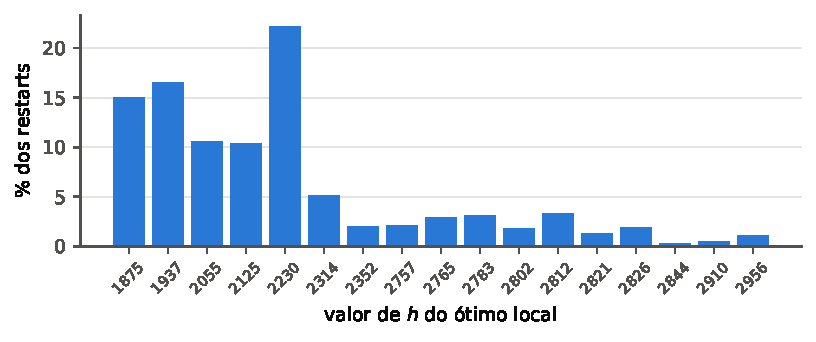
\includegraphics[width=0.75\linewidth]{figures/tp2/otimos_locais.pdf}
    \caption{Valores de $h$ dos ótimos locais atingidos pelo GD
    \textit{first} na instância pequena (\num{4088} \textit{restarts} somados
    nas 30 execuções).}
    \label{fig:otimos}
\end{figure}

\textbf{Exploração $\times$ intensificação.}
\begin{itemize}
    \item \textbf{GD.} A exploração vem só do \textit{random restart}, e a
    intensificação, da descida. Em $n=12$ esse equilíbrio é adequado, com
    136 reinícios por execução. Em $n=150$ ele colapsa: o GD \textit{first}
    gasta todo o orçamento em praticamente uma única descida (1 reinício,
    \num{1226} passos), e o GD \textit{best} não termina nem a primeira
    (13 passos). Nesse caso, a exploração não existe.
    \item \textbf{SA.} A exploração vem da aceitação de pioras quando $T$ é
    alta, e a intensificação, do regime frio no final. A
    \autoref{fig:sa} mostra a transição: a aceitação de pioras começa em
    49\%, 78\% e 28\% (pequena, intermediária e grande) e cai a 0\% antes da
    metade do orçamento, de modo que a segunda metade é \textit{greedy
    descent}. Na instância grande, a calibração escolheu $\chi_0=0{,}2$, ou
    seja, começar \emph{longe} do \textit{random walk}. Com
    \num{300000} avaliações para $n=150$, gastar o início em passeio aleatório
    deixa pouco orçamento para intensificar; o $\chi_0=0{,}8$ teve mediana
    \num{69715}, contra \num{67586} (Anexo~\ref{anexo:calib}). Ainda assim,
    a diferença entre as configurações é pequena diante da dispersão com 5
    execuções.
    \item \textbf{GA.} A exploração vem da mutação e da população, e a
    intensificação, da seleção e do elitismo. A \autoref{fig:div} mostra que
    \textbf{não houve convergência prematura}: ao fim do orçamento ainda há
    30--35 cromossomos distintos em 50, com distância de Hamming posicional
    média de cerca de 0,48. Na \autoref{fig:conv}, a média da população fica
    entre 11\% e 35\% acima do melhor indivíduo. O desequilíbrio é o oposto: a
    exploração é excessiva e a intensificação, fraca. O melhor $h$ estaciona
    (na pequena, em 1937, o 2.º ótimo local mais frequente) enquanto a
    população continua diversa, e os filhos gerados com $P_m=0{,}5$ quase
    sempre pioram. Taxas de mutação menores chegaram a ser testadas na
    calibração e não melhoraram o resultado.
\end{itemize}

\begin{figure}[H]
    \centering
    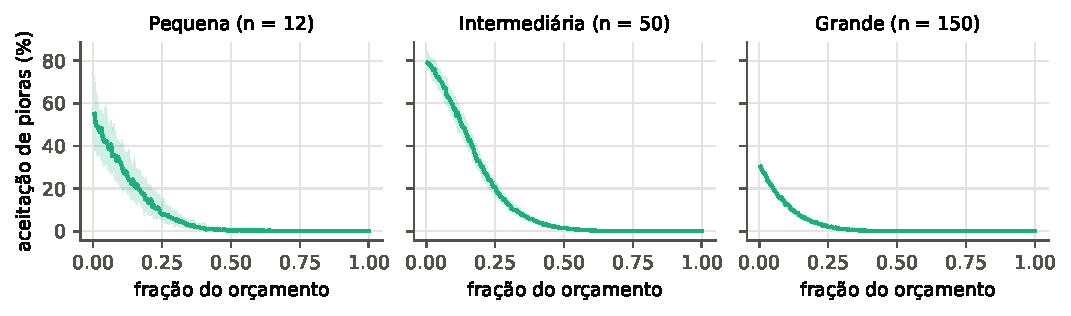
\includegraphics[width=\linewidth]{figures/tp2/sa_aceitacao.pdf}
    \caption{Taxa de aceitação de movimentos piores no SA, em janelas de 0,5\%
    do orçamento: mediana entre execuções, com a faixa entre os percentis 10 e
    90.}
    \label{fig:sa}
\end{figure}

\begin{figure}[H]
    \centering
    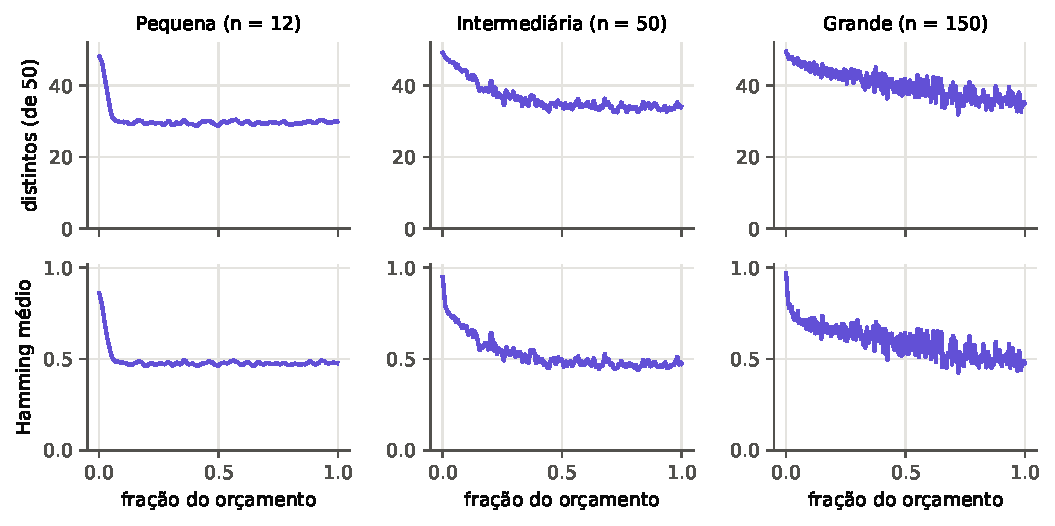
\includegraphics[width=\linewidth]{figures/tp2/ga_diversidade.pdf}
    \caption{Diversidade da população do GA: número de cromossomos distintos
    e distância de Hamming posicional média (normalizada) entre 200 pares
    sorteados. Mediana entre execuções, com média móvel de 25 gerações.}
    \label{fig:div}
\end{figure}

\textbf{Efeito da escala.} O \textit{ranking} muda com o tamanho da instância.
\begin{itemize}
    \item \textbf{Pequena:} GD (qualquer variante) e SA empatam no ótimo, e o
    GA fica atrás ($p<10^{-4}$).
    \item \textbf{Intermediária:} o SA supera o GD \textit{first}
    ($p=0{,}048$) e o GD aleatório ($p=0{,}002$); o GD \textit{best} cai para
    o mesmo patamar do GA.
    \item \textbf{Grande:} o SA vence com folga (mediana \num{71064} contra
    \num{82655}, $p=0{,}003$), o GD \textit{first} e o aleatório
    empatam ($p=0{,}91$), o GA \emph{deixa de ser significativamente pior} que
    o GD ($p=0{,}054$) e o GD \textit{best} é, de longe, o pior.
\end{itemize}

Nossa hipótese é que a escala atua por dois mecanismos:
\begin{enumerate}
    \item o custo de uma varredura cresce como $n^2$ e o orçamento só dobra
    de $n=50$ para $n=150$. A busca local que varre a vizinhança passa a
    caber em poucos passos (o \textit{best} dá 13), e a que não varre perde
    o \textit{restart}, que era o seu único mecanismo de exploração;
    \item com o espaço de busca muito maior ($150!$), o mecanismo de fuga
    \emph{dentro} de uma única trajetória, que é o do SA, passa a valer mais
    que reinícios independentes.
\end{enumerate}
O empate estatístico entre GA e GD em $n=150$ é efeito da piora do GD com a
escala, e não de uma melhora do GA.

\textbf{Quando o GA compensa?} Em nenhuma instância o GA superou as duas
abordagens de busca local; ele perde para o SA em todas ($p\le0{,}0006$).
Formulamos a hipótese de que a recombinação \emph{não} transmite bons trechos
de sequência nesta codificação. O custo de um ativo depende do seu
\emph{instante} de atendimento, isto é, de tudo o que vem antes dele. O OX
preserva um bloco de $p_1$ na posição original e a ordem relativa de $p_2$,
mas os genes de $p_2$ mudam de posição absoluta e, portanto, de instante:
um trecho bom em $p_2$ chega ao filho com outro prefixo e outro custo.

Para testar a hipótese, repetimos o GA com o protocolo completo em três
versões: com OX, com PMX (que mantém mais genes de $p_2$ na mesma posição
absoluta) e \textbf{sem cruzamento} ($P_c=0$, só mutação e seleção).

\begin{table}[H]
    \centering
    \caption{Experimento adicional: efeito do operador de cruzamento no GA
    (mesmo protocolo da Seção~3, mesmas sementes).}
    \label{table:extra}
    \begin{adjustbox}{max width=\linewidth}
    \begin{tabular}{llrrr}
\toprule
Instância & GA & média $\pm$ desvio & mediana & $p$ vs sem cruzamento \\
\midrule
Pequena ($n=12$) & OX & 2\,002 $\pm$ 154 & 1\,937 & 0,707 \\
 & PMX & 1\,937 $\pm$ 120 & 1\,875 & 0,015 \\
 & sem cruzamento ($P_c=0$) & 2\,017 $\pm$ 162 & 1\,937 & -- \\
\midrule
Intermediária ($n=50$) & OX & 19\,548 $\pm$ 1\,967 & 19\,636 & 0,469 \\
 & PMX & 19\,639 $\pm$ 2\,229 & 19\,212 & 0,501 \\
 & sem cruzamento ($P_c=0$) & 20\,001 $\pm$ 2\,058 & 19\,496 & -- \\
\midrule
Grande ($n=150$) & OX & 89\,739 $\pm$ 8\,316 & 91\,501 & 0,121 \\
 & PMX & 91\,249 $\pm$ 10\,311 & 89\,978 & 0,121 \\
 & sem cruzamento ($P_c=0$) & 84\,131 $\pm$ 5\,818 & 83\,983 & -- \\
\bottomrule
\end{tabular}

    \end{adjustbox}
\end{table}

A \autoref{table:extra} sustenta a hipótese:
\begin{itemize}
    \item nas instâncias intermediária e grande, nem o OX nem o PMX melhoram
    significativamente o GA sem cruzamento ($p\ge0{,}12$). Em $n=150$ a versão
    \emph{sem} cruzamento tem até a melhor mediana (\num{83984}, contra
    \num{91501} com OX). Ali o cruzamento consome orçamento sem contribuir, e
    o GA funciona como uma busca local populacional cara;
    \item o único ganho significativo é o do PMX na instância pequena
    ($p=0{,}015$), coerente com o argumento: entre os dois operadores, é o que
    mais preserva posições absolutas.
\end{itemize}
Para o GA compensar, a recombinação precisaria respeitar o que determina o
custo: operadores baseados em posição ou instante (PMX, \textit{position-based
crossover}), ou uma hibridização com a busca local (algoritmo memético). Ambos
ficam como trabalhos futuros.

% =========================================================================
\section{Conclusões}
% =========================================================================

Com orçamento fixo de avaliações:
\begin{itemize}
    \item o \textbf{SA} foi o melhor algoritmo nas instâncias intermediária e
    grande, com diferença estatisticamente significativa, e empatou no ótimo
    na pequena;
    \item o \textbf{GD} com \textit{random restart} resolve a instância
    pequena de forma trivial, mas perde a exploração conforme $n$ cresce;
    \item o \textbf{GA}, com a codificação por permutação e o OX, não
    aproveitou a recombinação.
\end{itemize}
O fator mais importante para o desempenho foi o casamento entre a vizinhança
e a estrutura do problema (a \textit{insertion}, que move um único ativo no
tempo), mais do que a escolha da metaheurística.
